% This file demonstrates how to use the IEEEConf LaTeX2e macro package,
% to prepare a manuscript for proceedings on CD of the conference
% FedCSIS
%
\documentclass[a4paper,10pt]{IEEEtran}
%\documentclass[a4paper]{IEEEconf}



% Usepackages
%%%%%%%%%%%%%%%%%%%%%%%%
%Article stuff
%%%%%%%%%%%%%%%%%%%%%%%%
% This package serves to balance the column lengths on the last page of the document.
% please, insert \balance command in the left column of the last page
\usepackage{balance}
\usepackage{supertabular}
\usepackage{paralist}

%% to enable \thank command
\IEEEoverridecommandlockouts 
%% The usage of the following packages is recommended
%% to insert graphics
\usepackage[dvips]{graphicx}
% to typeset algorithms
\usepackage{algorithm}
\usepackage{algpseudocode}
% to typeset code fragments
\usepackage{listings}
% to make an accent \k be available
\usepackage[T1]{fontenc}
% provides various features to facilitate writing math formulas and to improve the typographical quality of their output.
\usepackage[cmex10]{amsmath}
\interdisplaylinepenalty=2500
% por urls typesetting and breaking
\usepackage{url}
% for vertical merging table cells
\usepackage{multirow}
\usepackage{siunitx}


%%%%%%%%%%%%%%%%%%%%%%%%
%Mixed packages
%%%%%%%%%%%%%%%%%%%%%%%%
\usepackage[hidelinks]{hyperref}
\usepackage{graphicx}
\usepackage[textsize=scriptsize]{todonotes}
\usepackage{glossaries}
\usepackage[numbers]{natbib}
\usepackage{subcaption}
\bibliographystyle{plainnat}
\usepackage{amssymb}
\let\labelindent\relax %Needed before enumitem to avoid error with IEEE template
\usepackage{enumitem}
% Encoding %
\usepackage[utf8]{inputenc}

%%%%%%%%%%%%%%%%%%%%%%%%
%Figures
%%%%%%%%%%%%%%%%%%%%%%%%

\usepackage{tikz}
\usepackage{pgfplots}

% Tables %
\usepackage{tabularx}
\newcolumntype{Y}{>{\centering\arraybackslash}X}
\usepackage{booktabs} % for professional tables
\usepackage{tikz}
\usetikzlibrary{positioning}

%%%%%%%%%%%%%%%%%%%%%%%%
%Defines
%%%%%%%%%%%%%%%%%%%%%%%%

% Autoref
\def\sectionautorefname{Section}
\def\subsectionautorefname{Section}
\def\subsubsectionautorefname{Section}
\def\figureautorefname{Fig.}


% Macros
%%%%%%%%%%%%%%%%%%%%- Commands -%%%%%%%%%%%%%%%%%%%%%%%%%%%%%
\newcommand{\langballe}[2][]{\todo[color = cyan, #1]{\textbf{Langballe:} #2}}
\newcommand{\vejleder}[2][]{\todo[color = magenta, #1]{\textbf{Vejleder:} #2}}
\newcommand{\simba}[2][]{\todo[color = green, #1]{\textbf{Simba:} #2}}
\newcommand{\dennis}[2][]{\todo[color = pink, #1]{\textbf{Dennis:} #2}}


% Glossaries
\newacronym{Cluster-CMRW}{Cluster-CMRW}{Cluster-based Conditional Markov Random Walk Model}
\newacronym{lda}{LDA}{latent Dirichlet allocation}
\newacronym{NLP}{NLP}{Natural Language Processing}
\newacronym{lm}{LM}{language model}

%Glossary changes
%%%%%%%%%%%%%%%%%%%%%%%%
% Switch off hyperlinks for all uses of \gls etc.
% Hyperlinks will be inserted manually in the custom display style
\setkeys{glslink}{hyper=false}

\renewcommand*{\CustomAcronymFields}{%
	name={\the\glsshorttok},%
	description={\the\glslongtok},%
}

\renewcommand*{\SetCustomDisplayStyle}[1]{%
	\defglsentryfmt[#1]{%
		\ifdefempty\glscustomtext
		{%
			\ifglsused\glslabel
			{% subsequent use
				% Assuming all acronyms are written in upper case, so
				% not bother to check for case changes.
				\glsifplural
				{% subsequent use, plural
					\glshyperlink[\glsentryshortpl{\glslabel}]{\glslabel}%
				}%
				{% subsequent use, singular
					\glshyperlink[\glsentryshort{\glslabel}]{\glslabel}%
				}%
			}%
			{% first use
				\glsifplural
				{% first use, plural
					\glscapscase
					{% no case change
						\glstarget{\glslabel}{\glsentrylongpl{\glslabel}\glsinsert}%
						\space(\glsentryshortpl{\glslabel})%
					}%
					{% first letter upper case
						\glstarget{\glslabel}{\Glsentrylongpl{\glslabel}\glsinsert}%
						\space(\glsentryshortpl{\glslabel})%
					}%
					{% all caps
						\glstarget{\glslabel}{\MakeTextUppercase{%
								\glsentrylongpl{\glslabel}\glsinsert}}%
						\MakeTextUppercase{\space(\glsentryshortpl{\glslabel})}%
					}%
				}%
				{% first use, singular
					\glscapscase
					{% no case change
						\glstarget{\glslabel}{\glsentrylong{\glslabel}\glsinsert}%
						\space(\glsentryshort{\glslabel})%
					}%
					{% first letter upper case
						\glstarget{\glslabel}{\Glsentrylong{\glslabel}\glsinsert}%
						\space(\glsentryshort{\glslabel})%
					}%
					{% all caps
						\glstarget{\glslabel}{\MakeTextUppercase{%
								\glsentrylong{\glslabel}\glsinsert}}%
						\MakeTextUppercase{\space(\glsentryshort{\glslabel})}%
					}%
				}%
			}%
		}%
		{% \glsdisp used
			\ifglsused\glslabel
			{% subsequent use
				\glshyperlink[\glscustomtext]{\glslabel}%
			}%
			{% first use
				\glstarget{\glslabel}{\glscustomtext}%
			}%
		}%
	}%
}

\SetCustomStyle


%
%
\title{Improving Search using a combination of Random Walk and Topic Modeling}
%
%
\author{
\IEEEauthorblockN{Dennis Højbjerg Rose, Peter Langballe Erichsen, and Rasmus Engesgaard Christensen}\\
\IEEEauthorblockA{Department of Computer Science, Aalborg University,\\Selma Lagerløfs Vej 300, 9220 Aalborg Øst, Denmark\\Email: \{drose16, perich16, rech16\}@student.aau.dk}}

% conference papers do not typically use \thanks and this command
% is locked out in conference mode. If really needed, such as for
% the acknowledgment of grants, issue a \IEEEoverridecommandlockouts
% after \documentclass

% for over three affiliations, or if they all won't fit within the width
% of the page, use this alternative format:
% 
%\author{\IEEEauthorblockN{Michael Shell\IEEEauthorrefmark{1},
%Homer Simpson\IEEEauthorrefmark{2},
%James Kirk\IEEEauthorrefmark{3}, 
%Montgomery Scott\IEEEauthorrefmark{3} and
%Eldon Tyrell\IEEEauthorrefmark{4}}
%\IEEEauthorblockA{\IEEEauthorrefmark{1}School of Electrical and Computer Engineering\\
%Georgia Institute of Technology,
%Atlanta, Georgia 30332--0250\\ Email: see http://www.michaelshell.org/contact.html}
%\IEEEauthorblockA{\IEEEauthorrefmark{2}Twentieth Century Fox, Springfield, USA\\
%Email: homer@thesimpsons.com}
%\IEEEauthorblockA{\IEEEauthorrefmark{3}Starfleet Academy, San Francisco, California 96678-2391\\
%Telephone: (800) 555--1212, Fax: (888) 555--1212}
%\IEEEauthorblockA{\IEEEauthorrefmark{4}Tyrell Inc., 123 Replicant Street, Los Angeles, California 90210--4321}}

% \usepackage{showframe}
\begin{document}
\maketitle              % typeset the title of the contribution

% - Abstract (5-20 lines)
\begin{abstract}
	Topic models are used to discover topics within a set of documents.
In this paper, we investigate whether using a topic model can improve existing \acrlong{ir} methods.
We employ the probabilistic topic model, \acrlong{lda}, to automatically extract topics from Danish news articles.
%How can \gls{pr} be used on a dataset without explicit edges?
We use \acrlong{lda}, to construct an adjacency matrix, by measuring the Jensen-Shannon distance between the articles' topic distributions.
We test various \acrlong{ir} methods' ability to find documents related to a query, but also to find documents related to topics expressed in queries.
We evaluate \gls{ir} performance of combinations of \gls{lda}, \gls{tf-idf}, \gls{bm25}, \gls{lm}, and \gls{pr}.

\end{abstract}
\glsresetall
%\input{sections/Simba.tex}
%  Keywords
%\input{sections/Keywords.tex}
%
%\glsresetall
%
%% - Introduction (7.5 \%) 
\section{Introduction} 
%% Argue briefly for the relevance of the studied area/problem — start from general and end with your concrete problem.


Many news articles are produced every day and the need for searching the news is becoming a more prominent and difficult task.
A general challenge for search engines, no matter the environment, is how to acquire relevant search results from a given corpus. 
While some engines use simple algorithms, such as finding all articles that include a given search term and sorting by date, this may not always provide useful results.
Information retrieval within search engines apply many different techniques for either ranking or filtering documents\cite{google_pagerank2006}.

In order to rank these documents, some information is needed to support the underlying ranking.
A popular way to extract this information is through the use of topic modeling.
Topic modeling is a method within machine learning and \gls{NLP} which builds a model that can find abstract topics within a corpus of text documents.
A topic model assigns a distribution of topics to each document in a corpus, which can be used for different applications.
More specifically, we look into \gls{lda} since it is currently the most used topic model, and is applicable for many situations\cite{lda}.
\gls{lda} uses Dirichlet distributions to calculate the probability of a word belonging to a given topic and a document containing a given topic.
Topic modeling does not rank documents, which is why an additional part is necessary if we want to search the documents.

Ranking articles is a common \gls{ir} task and has been done in many ways.
One commonly used method is \gls{pr}\cite{google_pagerank2006}.
PageRank\cite{pagerank_1999} is a ranking algorithm, which is based on a random walk process.
The principle is to let a number of surfers walk between nodes in a graph, where each surfer takes one step in each iteration.
After an appropriate number of steps, the number of surfers on each node will be the ranking of the given node, where more surfers give a higher rank.
The edges in the graph can be based on many interactions, such as hyperlinks, similarities, genres, etc.

In \cite{yang2009topic} \citeauthor{yang2009topic} investigate how to combine topic model \gls{lda}, \gls{lm}, and PageRank.
They also investigate a modified version of the PageRank algorithm which takes topic-level information into account.
They use a scientific article dataset where they manually label 200 articles from their dataset based on related queries. 
In this paper, we want to expand the framework which \cite{yang2009topic} have provided.
However, the data set which \cite{yang2009topic} uses is based on scientific articles, which includes citation to other similar articles.
This citation scheme does not necessarily extent to other document types, such as news articles.
In this paper, we want to investigate whether using a similarity measure based on the topics generated by a topic model can be used with PageRank to improve \gls{ir} methods.

The combination of \gls{lda} and PageRank is interesting, since underlying document topics can yield more information than usually given by a single document.
These topics can be seen as sets of words shared between documents. 

When evaluating search engines, manual labeling of documents is usually used to measure the performance of models\cite{yang2009topic}\cite{Tang2008}.
Since the topics, created by the \gls{lda}, are distributions of words in documents, we can use these to evaluate a search algorithm's retrieval performance. 

Our goal is thus to improve news article search by using a combination of \gls{lda} and PageRank.
For our experiments we use the Nordjyske database of news articles as our dataset.
We also want to investigate whether an automatic evaluation measure can be used to evaluate a search engine.
Here we want to look into whether it makes sense to make an evaluation metric based on whether search results are in a given topic.
Finally, since the news article dataset does not include connections between the articles, how PageRank can be run on this needs to be investigated.
With these goals we look at the following questions:

\begin{quote}
	\emph{How can information retrieval techniques be evaluated based on search queries?}
	\begin{itemize}
		\item \emph{How can queries be generated for a dataset?}
		\item \emph{How can evaluation be done in a way that favors abstraction, rather than word frequency?}
	\end{itemize}
\end{quote}
\vspace{0.1 cm}

\begin{quote}
	\emph{How can PageRank be used on a document dataset with no connections between documents?}
\end{quote}

These questions also emphasize the contributions this paper brings.
We implement a method for constructing an adjacency matrix in order to run \gls{pr}, with no previous information given about connections between the nodes.
This is done by calculating the topic similarity between each document, using Jensen-Shannon distance, and using these similarities as the elements in the matrix.
We also suggest ways to measure the performance of an \gls{ir} method which has to find both specific documents and documents that share a specific topic.
Our system can be used to improve query results for search engines, by introducing a more abstract view of topics within a search query.

The paper is organized as follows:
In \autoref{sec:related-works}, articles related to topic modeling and random walk are investigated.
In \autoref{sec:method}, the theory behind LDA and clustering PageRank is detailed, and the pipeline is described.
\autoref{sec:experiment}
\autoref{sec:discussion}
\autoref{sec:conclusion} and \autoref{sec:future_work}

%
%% - Related works (7.5 \%))
\section{Related Work}\label{sec:related-works} \vejleder[inline]{add some more}
In this section, we investigate existing literature concerning \gls{lda} and similar topic models, as well as relevant work related to random walk.

\citet{lda} describes \acrlong{lda}, a generative statistical model, which is widely used within the field of topic modeling. 
The intuition behind the \gls{lda} topic model is that a document has an underlying distribution of topics, and that the words of a document are based on these topics.
We provide an overview of this model in \autoref{sec:lda}.

There also exists a large amount of extensions to \gls{lda}.
\citet{blei2012topicmodels} describes some of the most significant extensions that are made from relaxing the assumptions of \gls{lda}.
Some extensions mentioned are: the dynamic topic model\cite{blei2006dynamic} which assumes that topics change over time, and thus respects the order of the documents, and the correlated topic model\cite{blei2007correlated} and pachinko allocation model\cite{li2006pachinko} which each allow correlations to exist between topics.


\citet{quanti} describes a method of how to quantitatively preprocess and analyze large amounts of journalistic data dating from 1945-2000. 
They propose \gls{lda} as a way of categorizing articles and using this as the basis for search.
However, they only check for a single subject, namely the nuclear topic.  


\citet{Tang2008} successfully combine the two research fields of Topic Modeling and Random Walk search. 
Though their focus is mainly on mapping author and venue relations as part of their topic model, their methods for combining these two fields are still novel and generally applicable.


\citet{yang2009topic} presents a method for doing the topic-level random walk to search scientific articles.
\todo[inline]{mention LM and reference section}.
They also describe various combinations of \gls{lda} and PageRank.
These combinations are evaluated against information retrieval baselines such as BM25\cite{bm251996}.


This paper is largely based on the work of \citeauthor{yang2009topic}\cite{yang2009topic} and \citeauthor{Tang2008}\cite{Tang2008}.
However, the novelty in this paper comes from a different focus as described by our goals in \todo{ref introduction / goals}.
Our method will have the significant change of working with a new dataset consisting of documents without explicit connections between documents, which introduces a challenge in using PageRank effectively.
We also evaluate \gls{ir} performance based on queries generated from our dataset.

%Articles, we might want in our related works section:
%\begin{itemize}
%	\item \cite{lda} (written)
%	\item \cite{ClusterPageRank} (written)
%	\item \cite{Tang2008} (written)
%	\item \cite{jelodar2019latent}
%\end{itemize}

%
%% - Preliminaries/"Experiment" (20 \%)
%%		- Data
%%		- Setup
%%		- Analysis
\section{Dataset}\label{sec:dataset}
Nordjyske is a media group maintaining many local newspapers, radios, and websites in the North Jutland region of Denmark.
All articles produced by Nordjyske are saved in a nonpublic database.
The dataset, which we use, consists of $\sim$$63.000$ articles from 2017.
These documents consist of many attributes where we extract the ID, headline, and body of the article.
They do contain more information, such as authors, references to images, article type, date and time of publishing, etc.
This information could become relevant with the use of various \gls{lda} modifications, however this is beyond the scope of this paper.
Some entries within the dataset are advertisements or scoreboards, which we try to filter away in the preprocessing phase, explained in \autoref{sec:prepro}.
Before any preprocessing is applied, the average length of an articles is $231$ words.
The smallest article consists of only $2$ words and the biggest article is $3209$ words.

An example article can be seen in \autoref{prepro:example1}.

\begin{figure}[h]
	\begin{framed}
		\begin{quote}
			\textbf{headline:} \textit{'Tricktyve fik fingre i dankort HOBRO:'}\\
			\textbf{body:} \textit{'Frække tricktyve har atter slået til i en af Hobros dagligvareforretninger. Denne gang gik det ud over en 87-årig mand, som under indkøbsturen i Superbrugsen i Adelgade blev frastjålet sit Visa-Dankort med tilhørende pin-kode.'}
		\end{quote}
	\end{framed}
		\caption{Snippet of extracted information of an article in our dataset.}
		\label{prepro:example1}
\end{figure}

\section{Pipeline}

\tikzstyle{process} = [rectangle, rounded corners, minimum width=2cm, minimum height=1cm,text centered, draw=black, fill=gray!50]

\begin{figure}[h]
    \centering
    \begin{tikzpicture}[node distance=1.5cm]
    %\draw[step=1cm,gray,very thin] (-8,-8) grid (8,8);
	\node (Dataset) [process] {Article dataset};
	\node (Cleaning)[process, below of=Dataset] {Preprocessing Phase};
	\node (Training) [process, below of=Cleaning] {LDA};
	\node (Cluster PR) [process, below of=Training] {Clustering PageRank};
	\node (Query) at (-3.5, -4.5) [process] {Query Processing};
	\node (Result) [process, below of=Cluster PR] {Results};
	\draw [->, very thick] (Dataset) edge (Cleaning); 
	\draw [->, very thick] (Cleaning) edge (Training);
	\draw [->, very thick] (Training) edge (Cluster PR);
	\draw [->, very thick] (Cluster PR) edge (Result);
	\draw [->, very thick] (Query) edge (Cluster PR);
\end{tikzpicture}
	\caption{Pipeline}
    \label{fig:pipeline}
\end{figure}
The pipeline of our framework is divided into five phases which are displayed in \autoref{fig:pipeline}. \vejleder[inline]{???? how does that go together???	confusing structure }

\subsection{Article dataset}
We have a dataset consisting of articles from the media group Nordjyske. Their primary focus is to maintain a variety of local newspapers within the North Jutland region of Denmark. 
The data ranges from 2017-2019, where a total of $\sim$270.000 articles have been extracted from their database.

\subsection{Preprocessing Phase}
The extracted articles use the format:
\begin{itemize}
	\item id
	\item headline
	\item body
\end{itemize}
When training the LDA model, we concatenate the \emph{headline} and \emph{body} for simplicity. \vejleder[inline]{this sentence needs to be moved to another section, it does not match the subsection}
The preprocessing phase is described in further detail in \autoref{sec:prepro}.
This phase applies different \gls{NLP} methods \vejleder[inline]{DETAILS!} to simplify the dataset and remove redundant information.
After the preprocessing phase, we are left with $\sim$130.000 articles.

\subsection{LDA}
We apply the \acrfull{lda} to the dataset to generate topic clusters based on the content of the articles. 
We describe the investigation and selection of hyper parameters in \autoref{subsec:lda}. 
After the model has been trained, we have a document-topic distribution matrix $\theta$ and a topic-word distribution matrix $\beta$.
$\theta$ will be used as clusters in the next phase.

\subsection{Cluster-based PageRank}
In this phase, we apply cluster-based random walk, described in \autoref{sec:cluster_pagerank}, to the articles and clusters given in the \gls{lda} phase.
The algorithm yields a prioritized list of articles based on the query provided.


\subsection{Query Preprocessing}
The query \vejleder[inline]{basics missing I assume we’re talking about keywords} given to the search algorithm is stemmed and turned into a list of words. 
This list of words are then queried against LDA to check which cluster each word belongs to.
Lastly it is transformed into a personalization vector to use within the cluster-based PageRank.

%
\section{Preprocessing}\label{sec:prepro}

In this section, we will give a detailed overview of our method of preprocessing documents.
Our preprocessing steps were inspired by \cite{quanti}, who do a thorough preprocessing before applying LDA. 
Our preprocessing consists of several steps, each of which will be described in more detail, along with a running example over part of a real document.
The preprocessing steps are:
\begin{enumerate}[label=\alph*]
	\item Article Extraction
	\item Initial Document Filtering
	\item Stopword and Word Frequency Filtering
	\item Word Databases
	\item Stemming
	\item Construct Files
\end{enumerate}

\begin{table}
	\begin{tabular}{c|c|c}
		Preprocessing Step & Documents & Words\\
		Article Extraction & 63266 & unknown \\ 
		Initial Document Filtering & 32201 & 190133 \\ 
		Stopword and Word Frequency Filtering & 32201 & 16406 \\
		Word Databases & 32201 & 14537 \\
		Lemmatization & 32201 & 9934\\
	\end{tabular}
	\label{tab:prepro_doc_word}
	\caption{Amount of documents and unique words remaining after each preprocessing step.}
\end{table}

\paragraph{Article Extraction}
As described in \autoref{sec:dataset}, documents are loaded as \texttt{xml} files from the database, and their ID, title, and body contents extracted and converted into \texttt{json} format.
\autoref{prepro:example1} shows an example of an extracted document.
\begin{figure}[h]
	\begin{quote}
		\textit{
			'Tricktyve fik fingre i dankort HOBRO: Frække tricktyve har atter slået til i en af Hobros dagligvareforretninger. Denne gang gik det ud over en 87-årig mand, som under indkøbsturen i Superbrugsen i Adelgade blev frastjålet sit Visa-Dankort med tilhørende pin-kode.'
		}
	\end{quote}
	\caption{snippet of raw document}
	\label{prepro:example1}
\end{figure}

\paragraph{Initial Document Filtering}
The database contain many duplicate documents with the same content but different file names, we therefore start this phase by removing all duplicates.
All punctuation, numbers, and other non-alphabetic symbols are removed, keeping only words entirely made of alphabetic symbols.

Afterward, we remove documents containing fewer than 25 words.
This is done to remove ads, sports results, snippets, or other similar small sections that are present in newspapers but aren't really news articles.
\autoref{prepro:example2} shows an example of a document that would be removed. In this example, the document is merely a front-page snippet referencing an actual article, rather than a full news article.
\begin{figure}[h]
	\begin{quote}
		\textit{
			'Legedag for børnene Frivillighuset i Pandrup holdt for femte gang Legedag, så alle børn kan fortælle om en god ferieoplevelse. Side 12-13'
		}
	\end{quote}
	\caption{Example of document filtered for being too short}
	\label{prepro:example2}
\end{figure}

%\begin{quote}
%	\textit{
%		'tricktyve fik fingre i dankort hobro frække tricktyve har atter slået til i en af hobros dagligvareforretninger denne gang gik det ud over en årig mand som under indkøbsturen i superbrugsen i adelgade blev frastjålet sit visa dankort med tilhørende pin kode% inden kortet blev spærret nåede tyvene at hæve kr i en jutlander bank automat i hobro og yderligere et beløb i en billetautomat på århus kanten'
%	}
%\end{quote}

\paragraph{Stopword and Word Frequency Filtering}
Stopwords are removed, using \emph{nltk.corpus.stopwords}. We also added some stopwords ourselves based on manual inspection of words that appeared in close to every topic and had a high topic probability for multiple topics.
We also remove words based on their frequency. 
Words are removed if they appear fewer than 25 times.
These words are considered too rare to be relevant for a topic, as few documents will share these words.
Words are also removed if they appear in over 25\% of the documents.
These words are considered too common to be bound to specific topics and are therefore practically stop words.
These constants were the same used by \cite{quanti}.
\autoref{prepro:example3} shows how the document from \autoref{prepro:example1} has changed after this step.
\begin{figure}[h]
	\begin{quote}
		\textit{
			'fik fingre dankort hobro atter slået hobros gang gik årig mand superbrugsen adelgade dankort tilhørende kode'
		}
	\end{quote}
	\caption{Document from \autoref{prepro:example1} after removing stopwords and applying word frequency filtering.}
	\label{prepro:example3}
\end{figure}


\paragraph{Words Database Filtering}
Due to a lack of danish POS-tagging resources, we instead check up the words in our document set against two databases containing only words of specific word classes, namely: nouns, adjectives, verbs, adverbs, and proper nouns.
In practice this has the same effect as POS-tagging however words are not marked with their words class, instead they are removed if they do not appear in at least of the databases (containing only words of approved word classes).
The two databases used are:  Wiktionary\footnote{https://github.com/fnielsen/awesome-danish (specifically Danish resources: https://people.compute.dtu.dk/faan/ps/Nielsen2016Danish.pdf)} and DanNet\cite{Pedersen2009DanNetTC}. 

Most words remaining at this step are contained within the databases, so this step does not remove as many words, however, this is mostly due to the step being taken late, due to having a longer computation time per word.
This step mostly serves to remove names, and words from different languages, namely English.
However, does also cut the odd non-word (eg. 'gimi') and abbreviations (eg. 'DK') that still exists at this point in the preprocessing.
The example used in \autoref{prepro:example3} does not change at this step. 
Instead, \autoref{prepro:example4} shows an example of another document that does change during this step.

\begin{figure}[h]
	\begin{quote}
		\textit{
			'\colorbox{pink}{country} kræver sommerens by \colorbox{pink}{night} sluttede afslappet band'
		}
	\end{quote}
	\caption{Snippet of a document which had words removed during the word database filtering.}
	\label{prepro:example4}
\end{figure}

\paragraph{Lemmatization}
Words are reduced to their stems using the python package \texttt{lemmy}. 
This is done by combining word inflections.
However since we do not have proper POS-tagging, some words have multiple different meaning depending on the word class. In these cases we keep all inflected words.
After lemmatization has been applied some words might have been converted into stopwords.
We, therefore, remove stopwords once again.
We also remove any potential documents that may have become empty after all the word filtering, however, this is usually not the case.
\begin{figure}[h]
	\begin{quote}
		\textit{
			'fingre dankort hobro atter årig adelgade dankort kode inden hæve bank hobro århus få slå hobro gange gang mande mand superbrugs tilhøre'
		}
	\end{quote}
	\caption{Lemmetized version of the example document from \autoref{prepro:example3}}
	\label{prepro:example5}
\end{figure}

\paragraph{Construct Files}
Construct and save \texttt{CountVectorizer} (word-document frequency matrix) as a sparse matrix \texttt{npz} file. This file is used by the LDA to construct a document-topic matrix and a topic-word matrix.
We also save various lookup files in \texttt{csv} format. \texttt{word2vec}, \texttt{doc2vec} files translate word and document to their ids.
\texttt{doc2word} translates document ids to all the ids of the words used in the document.
These files allow us to only use ids from here on, and then later translate back to words when needed.

%\subsection{Post-LDA Preprocessing}
%After LDA has made a topic model, documents which have no associated topics, and topics which have no associated documents would be removed.
%Topics that occur in almost every document are also considered too general, and would also be removed.
%Initially, this presented some implementation challenges, as it required removing topics and documents from files generated earlier in the process and from the LDA model, to be able to use the right topic/document IDs in the future.

\subsection{Query Preprocessing}
\todo[inline]{move this subsec to query section}
One of the challenges of preprocessing queries is that they usually contain very few words.
Therefore, there is a huge possibility of information loss during preprocessing and conversion, as there is not much content or context to be learned from.

Our method converts each word in the query into a topic distribution, making the query have the same format as a document. \todo[inline]{Detaljer specifikt hvordan denne distribution laves, når det er færdigimplementeret.}
This enables us to compare the query to other documents, and therefore do a random walk based on the query \vejleder[inline]{say why this is usefull}.
The danger of this method is that a query only containing a couple of words, will likely have a very skewed topic distribution.
\todo[inline]{make running example}

\subsection{\acrlong{lda}}\label{sec:lda}
\Gls{lda} is topic model method.
The objective of topic modeling is to infer topics (collections of words) in a document set.

\begin{definition}\label{def:topic}
	\textit{A topic is a distribution over words in a corpus.}
\end{definition}

The result consists of a topic-word distribution matrix $\beta$, which for each topic gives a distribution of words belonging to said topic, and a document-topic distribution matrix $\theta$ which for each document gives a distribution of topics to which the document belongs to.

\citet{lda} introduced \gls{lda}, which has since become a staple within topic modeling.
\gls{lda} works under the assumption that documents are generated from a specific generative process, and tries to reverse engineer this process.
This generative process assumes that documents are random mixtures of latent topics and that each topic is a distribution over all the words in the corpus.

This process generates $K$ topics and $D$ documents containing $N_{d}$ words, where $d$ is a document in $D$.
The generative process has two Dirichlet distributions $Dir(\alpha)$ for the document-topic relation and $Dir(\eta)$ for the topic-word relation.

\begin{figure}[h]
	\centering
	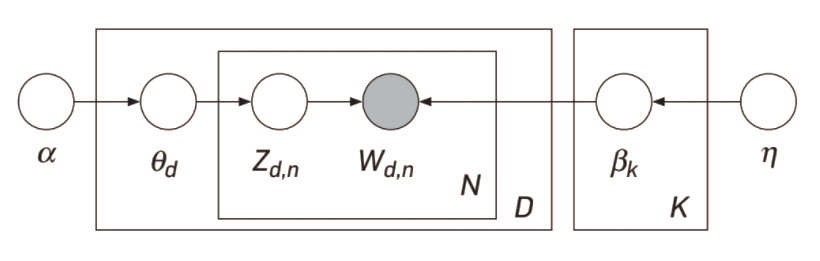
\includegraphics[width=0.5\textwidth]{figures/Smoothed_LDA.jpg}
	\caption{Plate notation for \gls{lda}. Boxes symbolize repeated processes, shaded elements are observed information. Image is from \citet{blei2012topicmodels}.}
	\label{fig:lda}
\end{figure}

From these Dirichlet distributions, we can sample two multinomial distributions: a document-topic distribution $\theta_d$ for each document $d$, and a topic-word distribution $\beta_k$ for each topic $k$.
$\theta$ and $\beta$ are stored as matrices.
These Dirichlet distributions are tuned with the hyperparameters $\alpha$ and $\eta$, which adjust the entropy of the sampled distributions.
An $\alpha$ value near 1 causes each document to be distributed over almost all topics, while an $\alpha$ value near 0 causes each document to be distributed over only a few topics.
Similarly $\eta$ will adjust how many words each topic contains.
This also has the added consequence that a high $\alpha$ will make documents appear more similar, and a high $\eta$ will make topics appear more similar.

Using $\theta$ and $\beta$, we can sample concrete topics $Z$ from documents, and concrete words $W$ from topics.
\autoref{fig:lda} gives an overview of the generative process.

\Gls{lda} has some underlying assumptions, which also explain its limitations\cite{blei2012topicmodels}:
\begin{itemize}
	\item \gls{lda} assumes ordering of words does not matter (Bag of Words).
	\item \gls{lda} assumes ordering of documents does not matter.
	\item \gls{lda} assumes that the number of topics is fixed and known.
\end{itemize}
However, many of these assumptions can be addressed through various extensions of the \gls{lda} model\cite{blei2012topicmodels}.

\subsubsection{\gls{lda}-\gls{ir}}\label{subsec:lda_ir}
\gls{lda} is not designed as an \acrlong{ir} method.
And as such, it usually gives subpar performance when applied to \gls{ir} tasks.
This is due to topic modeling working on the more abstract level of topics, rather than word frequencies as many of the other \gls{ir} methods.
However, this also gives \gls{lda} the ability to understand topics expressed in queries and do \gls{ir} based on that knowledge.

\citet{yang2009topic} defines \autoref{eq:lda-ir} for using \gls{lda} as an \gls{ir} method.
They do this based on a previous application of \gls{lda} for \gls{ir}\cite{lda-ir}.

\begin{equation}\label{eq:lda-ir}
	P(w|d, \theta, \beta) = \sum_{z \in T} P(w|z,\beta_z) P(z|d,\theta_d)
\end{equation}

The idea behind this equation is to reverse-engineer the generative process \gls{lda} uses to create the topic model, to predict the probability of a word appearing in a document given the document-topic distribution matrix $\theta$ and the topic-word distribution matrix $\beta$.
So, for each topic $z$, the probability of the word $w$ using $\beta_z$ is multiplied with the probability of that topic appearing in the document using $\theta_d$.

This is similar to the process \gls{lda} uses to generate topics, but instead of constructing topic-word distributions and document-topic distributions based on observed words, we now use these distributions and the observed words to find the probability of a word appearing in a document based on its topic distribution.
In practice, we multiply the $\theta$ and $\beta$ matrices together and get a $document \cdot word$ matrix, where each cell represents the probability of a given word appearing in a specific document w.r.t. the topic they share.
We use the term \gls{lda}-\gls{ir}, to refer to information retrieval made using \autoref{eq:lda-ir}.

\section{Cluster-based Random Walk}\label{sec:cluster_pagerank}
To perform random walk on a document set, such as Nordjyske, probabilities of jumping between documents is needed to perform each step. 
When performing a random walk, we get the articles that most important based on the information that the probabilities are based on. 
If it was based on word frequency, a random walk would return an ordered list of articles, where the ordering is based on the frequency of a given word.
 
We have chosen to use a similarity measure between each document as these probabilities.
This is calculated by using the document-topic distributions from the \gls{lda}.
These distributions can be arranged in a matrix $\theta$, which is described later.

In \cite{ClusterPageRank}, they describe the \gls{Cluster-CMRW} which is a new version of the random walk model. 
They improve upon this model by incorporating information from clusters. 
The clusters are found by employing three different clustering algorithms.
They create a new transition probability matrix where the cluster information is added by combining three similarity functions based on the information levels present in the data.
They describe three similarity levels between:
\begin{itemize}
    \item Sentence to Sentence - $f(v_i \rightarrow v_j)$
    \item Sentence to Topic Cluster - $\omega(v_i, clus(v_i))$
    \item Topic Cluster to Document Set - $\pi(clus(v_i))$
\end{itemize}
where $v_i$ is the given sentence and $clus(v_i)$ is the cluster that $v_i$ belongs to.

We want to use this method to incorporate the information given by the topic distributions within a \gls{Cluster-CMRW}. 
We first create three similarity functions to incorporate topic cluster level information into a new adjacency matrix.
\begin{itemize}
    \item Document to Document - $f(d_i \rightarrow d_j)$
    \item Document to Topic Cluster - $\omega(d_i,vlus(d_i))$
    \item Topic Cluster to Document Set - $\pi(clus(d_i))$
\end{itemize}
\todo{details}


\noindent
Where $d$ is a document, $clus(d_i)$ is a topic cluster of document $d_i$.
Notice that a document $d$ can contain multiple topics, as opposed to normal clustering where each element is generally assumed to only be part of one cluster.

\subsection*{Document to Document similarity}
We define the similarity of two articles as the distance between their distribution, which is calculated using square root of Jensen-Shannon divergence, which is often called Jensen-Shannon distance\cite{jensen-shannon2003}\cite{jensen-shannondis2003}.
This metric gives a score between 0-1 based on the distance between two distributions, where a low distance is equal to more similar.
So our similarity function is:
$$ f(d_i \rightarrow d_j) = 1 - \text{jenson-shannon-distance}(d_i, d_j)$$ 

\subsection*{Document to Topic Cluster similarity}
We define the similarity between a document and a topic cluster as the document-topic probability distribution between them.
$$ \omega(d_i,clus(d_i)) = \theta_{d_i,clus(d_i)}$$
where $\theta$ is the document-topic distribution matrix.

\subsection*{Topic Cluster to Document Set similarity}
We define the similarity between a topic $t$ and the whole document set as:
$$ \pi(clus(d_i)) = \frac{\sum_{d}^{M} \theta_{clus(d_i)}}{M} $$
where $M$ is the number of documents in the document set.


To create the adjacency matrix, \cite{ClusterPageRank} linearly combine the different similarity functions, in which we intend to do the same.
Formally, the adjacency matrix is calculated with the following function.
$$ f(d_i \rightarrow d_j | clus(d_i), clus(d_j)) $$
which is evaluated to 

\begin{align*}
&f(d_i \rightarrow d_j | clus(d_i), clus(d_j)) = \\
&f(d_i, d_j) \cdot (\lambda \cdot \pi(clus(d_i))) \cdot \omega(d_i, clus(d_i)) \\ 
&+ (1-\lambda) \cdot \pi(clus(d_j)) \cdot \omega(d_j, clus(d_j))
\end{align*}
where $\lambda$ is a weight between $[0,1]$ that controls the relative contribution of the two clusters.




%\section{Dataset}\label{sec:dataset}
Nordjyske is a media group maintaining many local newspapers, radios, and websites in the North Jutland region of Denmark.
All articles produced by Nordjyske are saved in a nonpublic database.
The dataset, which we use, consists of $\sim$$63.000$ articles from 2017.
These documents consist of many attributes where we extract the ID, headline, and body of the article.
They do contain more information, such as authors, references to images, article type, date and time of publishing, etc.
This information could become relevant with the use of various \gls{lda} modifications, however this is beyond the scope of this paper.
Some entries within the dataset are advertisements or scoreboards, which we try to filter away in the preprocessing phase, explained in \autoref{sec:prepro}.
Before any preprocessing is applied, the average length of an articles is $231$ words.
The smallest article consists of only $2$ words and the biggest article is $3209$ words.

An example article can be seen in \autoref{prepro:example1}.

\begin{figure}[h]
	\begin{framed}
		\begin{quote}
			\textbf{headline:} \textit{'Tricktyve fik fingre i dankort HOBRO:'}\\
			\textbf{body:} \textit{'Frække tricktyve har atter slået til i en af Hobros dagligvareforretninger. Denne gang gik det ud over en 87-årig mand, som under indkøbsturen i Superbrugsen i Adelgade blev frastjålet sit Visa-Dankort med tilhørende pin-kode.'}
		\end{quote}
	\end{framed}
		\caption{Snippet of extracted information of an article in our dataset.}
		\label{prepro:example1}
\end{figure}

%%\section{Pipeline}

\tikzstyle{process} = [rectangle, rounded corners, minimum width=2cm, minimum height=1cm,text centered, draw=black, fill=gray!50]

\begin{figure}[h]
    \centering
    \begin{tikzpicture}[node distance=1.5cm]
    %\draw[step=1cm,gray,very thin] (-8,-8) grid (8,8);
	\node (Dataset) [process] {Article dataset};
	\node (Cleaning)[process, below of=Dataset] {Preprocessing Phase};
	\node (Training) [process, below of=Cleaning] {LDA};
	\node (Cluster PR) [process, below of=Training] {Clustering PageRank};
	\node (Query) at (-3.5, -4.5) [process] {Query Processing};
	\node (Result) [process, below of=Cluster PR] {Results};
	\draw [->, very thick] (Dataset) edge (Cleaning); 
	\draw [->, very thick] (Cleaning) edge (Training);
	\draw [->, very thick] (Training) edge (Cluster PR);
	\draw [->, very thick] (Cluster PR) edge (Result);
	\draw [->, very thick] (Query) edge (Cluster PR);
\end{tikzpicture}
	\caption{Pipeline}
    \label{fig:pipeline}
\end{figure}
The pipeline of our framework is divided into five phases which are displayed in \autoref{fig:pipeline}. \vejleder[inline]{???? how does that go together???	confusing structure }

\subsection{Article dataset}
We have a dataset consisting of articles from the media group Nordjyske. Their primary focus is to maintain a variety of local newspapers within the North Jutland region of Denmark. 
The data ranges from 2017-2019, where a total of $\sim$270.000 articles have been extracted from their database.

\subsection{Preprocessing Phase}
The extracted articles use the format:
\begin{itemize}
	\item id
	\item headline
	\item body
\end{itemize}
When training the LDA model, we concatenate the \emph{headline} and \emph{body} for simplicity. \vejleder[inline]{this sentence needs to be moved to another section, it does not match the subsection}
The preprocessing phase is described in further detail in \autoref{sec:prepro}.
This phase applies different \gls{NLP} methods \vejleder[inline]{DETAILS!} to simplify the dataset and remove redundant information.
After the preprocessing phase, we are left with $\sim$130.000 articles.

\subsection{LDA}
We apply the \acrfull{lda} to the dataset to generate topic clusters based on the content of the articles. 
We describe the investigation and selection of hyper parameters in \autoref{subsec:lda}. 
After the model has been trained, we have a document-topic distribution matrix $\theta$ and a topic-word distribution matrix $\beta$.
$\theta$ will be used as clusters in the next phase.

\subsection{Cluster-based PageRank}
In this phase, we apply cluster-based random walk, described in \autoref{sec:cluster_pagerank}, to the articles and clusters given in the \gls{lda} phase.
The algorithm yields a prioritized list of articles based on the query provided.


\subsection{Query Preprocessing}
The query \vejleder[inline]{basics missing I assume we’re talking about keywords} given to the search algorithm is stemmed and turned into a list of words. 
This list of words are then queried against LDA to check which cluster each word belongs to.
Lastly it is transformed into a personalization vector to use within the cluster-based PageRank.

\section{Experiments}\label{sec:experiment}

\subsection{Results}\label{subsec:results}

\begin{table*}[h]
	\centering
	\caption{Results table}
	\begin{tabular}{l|c|c|c|c|c|c|c|c}
		Model / Mean Average Precision & D1 & D2 & D3 & D4 & T1 & T2 & T3 & T4 \\
		\midrule
		\gls{lda} & 0.00457 & 0.00527 & 0.0429 & 0.0538 & 0.155 & 0.186 & 0.168 & 0.178 \\
		\gls{lm} & 0.198 & 0.152 & 0.291 & 0.260 & 0.126 & 0.130 & 0.128 & 0.129 \\
		\gls{bm25} & 0.270 & 0.656 & 0.866 & \textbf{0.908} & 0.155 & 0.158 & 0.155 & 0.161 \\
		\gls{tf-idf} & 0.210 & 0.621 & 0.799 & 0.897 & 0.155 & 0.157 & 0.155 & 0.161 \\
		\gls{lda} + \gls{pr} & 0.00458 & 0.00526 & 0.0429 & 0.0538 & 0.162 & \textbf{0.195} & \textbf{0.177} & \textbf{0.187} \\
		\gls{lda} * \gls{pr} & 0.00781 & 0.00569 & 0.0410 & 0.0537 & 0.156 & 0.186 & 0.168 & 0.179 \\
		\gls{lm} + \gls{lda} & 0.0419 & 0.0214 & 0.0602 & 0.120 & 0.147 & 0.163 & 0.145 & 0.146 \\
		\gls{lm} * \gls{lda} & 0.0931 & 0.0462 & 0.175 & 0.177 & 0.150 & 0.175 & 0.155 & 0.166 \\
		\gls{lm} + \gls{pr} & 0.170 & 0.153 & 0.283 & 0.256 & 0.130 & 0.132 & 0.130 & 0.131 \\
		\gls{lm} * \gls{pr} & 0.163 & 0.138 & 0.259 & 0.236 & 0.130 & 0.133 & 0.129 & 0.130 \\
		\gls{bm25} + \gls{pr} & 0.269 & 0.656 & 0.866 & 0.902 & \textbf{0.192} & 0.193 & 0.175 & 0.183 \\
		\gls{bm25} * \gls{pr} & 0.267 & \textbf{0.663} & \textbf{0.884} & 0.904 & 0.155 & 0.159 & 0.155 & 0.161 \\
		\gls{bm25} + \gls{lda} + \gls{pr} & \textbf{0.276} & 0.525 & 0.589 & 0.366 & 0.162 & 0.192 & 0.176 & 0.184 \\
		\gls{bm25} * \gls{lda} * \gls{pr} & 0.150 & 0.266 & 0.446 & 0.381 & 0.155 & 0.159 & 0.156 & 0.163 \\
	\end{tabular}
	
	\label{tab:results}
\end{table*}


\begin{table*}[h]
	\centering
	\caption{Results table}
	\begin{tabular}{l|c|c|c|c||c|c|c|c}
		Model / P@10 || P@100 & T1 & T2 & T3 & T4 & T1 & T2 & T3 & T4\\
		\midrule
		\gls{lda} & 0.02 & 0.103 & 0.13 & 0.203 & 0.062 & 0.131 & 0.164 & 0.191 \\
		\gls{lm} & 0.126 & 0.118 & 0.116 & 0.069 & 0.090 & 0.092 & 0.087 & 0.093\\
		\gls{bm25} & 0.136 & 0.161 & 0.164 & 0.174 & 0.142 & 0.165 & 0.175 & 0.151\\ 
		\gls{tf-idf} & 0.16 & 0.125 & 0.2 & 0.148 & 0.163 & 0.169 & \textbf{0.188} & 0.170 \\
		\gls{lda} + \gls{pr} & 0.0188 & 0.103 & 0.141 & \textbf{0.211} & 0.062 & 0.131 & 0.175 & \textbf{0.198} \\
		\gls{lda} * \gls{pr} & 0.0125 & 0.100 & 0.133 & 0.200 & 0.062 & 0.132 & 0.167 & 0.192 \\
		\gls{lm} + \gls{lda} & 0.02 & 0.101 & 0.136 & 0.196 & 0.060 & 0.129 & 0.161 & 0.188  \\
		\gls{lm} * \gls{lda} & 0.02 & 0.085 & 0.109 & 0.161 & 0.055 & 0.114 & 0.129 & 0.152 \\
		\gls{lm} + \gls{pr} & 0.138 & 0.130 & 0.116 & 0.0763 & 0.110 & 0.108 & 0.097 & 0.098 \\
		\gls{lm} * \gls{pr} & 0.148 & 0.128 & 0.116 & 0.0963 & 0.110 & 0.112 & 0.101 & 0.101 \\
		\gls{lm} + \gls{lda} + \gls{pr} & 0.019 & 0.101 & 0.134 & 0.195 & 0.061 & 0.129 & 0.163 & 0.187\\
		\gls{lm} * \gls{lda} * \gls{pr} & 0.026 & 0.090 & 0.110 & 0.161 & 0.059 & 0.115 & 0.130 & 0.152\\
		\gls{bm25} + \gls{pr} & 0.135 & 0.163 & 0.165 & 0.173 & \textbf{0.155} & 0.165 & 0.176 & 0.151 \\
		\gls{bm25} * \gls{pr} & \textbf{0.165} & \textbf{0.169} & \textbf{0.184} & 0.170 & 0.148 & \textbf{0.177} & 0.186 & 0.161\\
		\gls{bm25} + \gls{lda} & 0.124 & 0.160 & 0.154 & 0.204 & 0.113 & 0.155 & 0.168 & 0.198 \\
		\gls{bm25} * \gls{lda} & 0.09 & 0.139 & 0.175& 0.206 & 0.134 & 0.170 & 0.174 & 0.187 \\
		\gls{bm25} + \gls{lda} + \gls{pr} & 0.124 & 0.160 & 0.154 & 0.204 & 0.113 & 0.155 & 0.17 & \textbf{0.198}\\
		\gls{bm25} * \gls{lda} * \gls{pr} & 0.095 & 0.141 & 0.176 & 0.206 & 0.135 & 0.174 & 0.174 & 0.188\\
	\end{tabular}
	
	\label{tab:results_precision_at_10}
\end{table*}


\begin{table}[h]
	\centering
	\caption{Average rank of relevant document for document-queries.}
	\begin{tabular}{l|c|c|c|c}
		Model / Avg. rank & D1 & D2 & D3 & D4 \\
		\midrule
		\gls{lda} & 2287.93 & 1599.95 & 1241.18 & 1926.78 \\
		\gls{lm} & 7120.04 & 9082.9 & 6501.85 & 7782.65 \\
		\gls{bm25} & \textbf{19.58} & 7.94 & 1.78 & 1.41 \\
		\gls{tf-idf} & 30.0 & 9.3 & 2.03 & 1.29 \\
		\gls{lda} + \gls{pr} & 2491.31 & 1342.53 & 1126.23 & 1906.76\\
		\gls{lda} * \gls{pr} & 2305.04 & 1600.93 & 1223.14 & 1920.175\\
		\gls{lm} + \gls{lda} & 1971.19 & 1192.91 & 1027.95 & 1482.69 \\
		\gls{lm} * \gls{lda} & 1874.81 & 1456.21 & 954.66 & 1853.44 \\
		\gls{lm} + \gls{pr} & 7299.85 & 9134.81 & 6429.24 & 7725.36 \\
		\gls{lm} * \gls{pr} & 7328.7625 & 9137.23 & 6504.85 & 7772.4\\
		\gls{lm} + \gls{lda} + \gls{pr} & 1978.74 & 1179.21 & 994.91 & 1438.88 \\
		\gls{lm} * \gls{lda} * \gls{pr} & 1892.12 & 1453.56 & 941.4 & 1850.43 \\
		\gls{bm25} + \gls{lda} & 30.45 & 28.59 & 17.7 & 23.76 \\
		\gls{bm25} * \gls{lda} & 163.76 & 557.13 & 297.48 & 1159.33 \\
		\gls{bm25} + \gls{pr} & 19.69 & \textbf{7.88} & 1.79 & 1.43\\
		\gls{bm25} * \gls{pr} & 23.96 & 8.45 & \textbf{1.61} & \textbf{1.24}\\
		\gls{bm25} + \gls{lda} + \gls{pr} & 30.35 & 28.44 & 17.65 & 23.76\\
		\gls{bm25} * \gls{lda} * \gls{pr} & 163.5 & 555.35 & 295.69 & 1158.08\\
	\end{tabular}
	
	\label{tab:hit_results}
\end{table}


\subsection{Hyperparameters}\label{subsec:hyperparameters}
Before setting up our experiment, we did some initial testing to find acceptable hyperparameter values for our \gls{lda} model.
% runtime parameters
First, we adjusted parameters that had to do with how the algorithms run to ensure that the model converged, without spending unnecessary resources.
\texttt{passes} adjusts how many times the model passes over the whole corpus, and can be seen as an 'epoch'. 
This is necessary for smaller datasets to ensure convergence before the algorithm finishes, but for large enough datasets this parameter can have a value of 1, as is the case for \cite{blei2010online} where their corpus includes 3.3M documents, where our dataset is $\sim$32000 documents.
\texttt{iterations} which adjusts the maximum number of iterations of the E-step (from \cite{}, Algorithm 2)\todo{cite} that are allowed without all documents having converged. 
Setting this to a high value ensures convergence, but also increases training time. 
In practice, iterations should be set to the lowest possible values where nearly all (> 99\%) documents have converged by the end of the training.
From testing we found 20 \texttt{passes} and 100 \texttt{iterations} was enough to converge 27678 out of 27919 documents (99.14\%).

% model parameters
Once we had assured convergence of our model, we tested hyperparameters for our \gls{lda} model.
These include:
\begin{itemize}
	\item K - the number of topics
	\item $\alpha$ - dirichlet prior for document-topic distributions
	\item $\eta$ - dirichlet prior for topic-word distributions
\end{itemize}
Similar to clustering algorithms, there is usually an optimal setting for K, where all values above will produce topics that are subtopics of the optimal topics, and all values below will achieve subpar performance.
This theoretical optimal value is however based on the corpus, so tests are needed to find some setting of K that is close to the optimal.
$\alpha$ and $\eta$ adjusts the Dirichlet distributions, which will create the multinomial distributions for document-topic and topic-word relations, respectively.
Lower values will lead to more uneven distributions, favoring fewer topics per document and fewer words per topic, while higher values will make the distribution more uniform.

To find the optimal hyperparameter values we did two sequential grid-searches using the hyperparameter values shown in \autoref{tab:params}.
The first grid-search used the values for $K_1$, while the second used the $K_2$ values.
In both grid-searches the same $\alpha$ and $\eta$ values are used.
To evaluate the \gls{lda} models, we measured perplexity \todo{explain perplexity}\todo{and explain how we choose our model by hand}.
During the first grid-search, we found that $10$ and $50$ were clearly the best values for K.
However, $\alpha$ and $\eta$ values showed no clear favorite.
For the second grid-search we choose more specific K values, to narrow the search, while keeping the $\alpha$ and $\eta$ values the same.
\todo[inline]{add graphs from gridsearches}

Based on manual inspection and evaluation of topics generated by the second grid-search we choose $K = 30$, $\alpha = 0.1$, and $\eta = 0.1$ as the hyperparameters for the final \gls{lda} model.
A new model is generated using these values and this model will be used for the whole experiment.

\begin{table}[h]
	\centering
	\begin{tabular}{c|c}
		Parameter & Tested Values\\
		\hline
		$K_1$ & 10, 50, 100, 200, 300\\
		$K_2$ & 5, 10, 15, 20, 25, 30, 35, 40, 45, 50\\
		$\alpha$ & 0.5, 0.1, 0.01, 0.001\\
		$\eta$ & 0.1, 0.01, 0.001, 0.0001\\
	\end{tabular}
	\caption{Tested hyperparameter values. $K_1$ is the $K$ values used for the first hyperparameter test, while $K_2$ is the $K$ values used for the second hyperparameter test.}
	\label{tab:params}
\end{table}

%% - Body(50 \%)
%%	- Results 
%
%%	- Discussion
%%		- Main results
%%		- Other results
%%		- Error sources
\section{Discussion}\label{sec:discussion}
In this section, we analyze and describe the results, we get from running our experiment.

\gls{pr} using our adjacency-matrix successfully improved upon the results of other models in many cases.
This is worth noting as our adjacency matrix was constructed based on similarity of the documents' topic-distributions, rather than any relation embedded in the documents themselves, such as scientific articles referencing each other as with \citeauthor{yang2009topic}\cite{yang2009topic}.
This suggests that other \gls{ir} methods benefit from the similarity context provided by our \gls{pr}, regardless of the validity of the underlying edges.
This means that our initial idea of using the topic distributions as a similarity measure in the \gls{pr} algorithm, was a success.
\todo[inline]{Vurdering af egen adjacency matrix som edges i PR i forhold til original paper. Hvis vi når det: generaliserbarhed af dette (andet datasæt)}

\gls{lm} performed surprisingly bad compared to the results of \cite{yang2009topic}. 
\todo[inline]{We need to figure out what we are going to say about lm's bad performance, or maybe move some of it to appendix if we want to avoid talking too much about it}

\gls{lda} gets good topic query retrieval results when combined with \gls{pr}, as seen in \autoref{tab:results}.
This comes at the cost of very bad document query retrieval results.
Though \gls{lda} has good \gls{map} results, \autoref{tab:results_precision_at_10} shows that \gls{lda} only gets the best precision@10 and precision@100 with queries of 4 words.
This means that while it is well suited for ranking a large number of documents fairly well (as with \gls{map}), it is not good at finding a relatively small number of relevant documents
It also points towards \gls{lda} being more reliant on a larger amount of context than many of the other models, and could therefore likely benefit greatly from query expansion methods.
However, for this experiment \gls{lda}'s purpose is mostly to improve the topic retrieval performance of other models it is combined with, at the cost of reducing their document retrieval performance.

Overall, the most successful combinations of baselines for combining document query retrieval and topic query retrieval seem to be $\gls{bm25}+\gls{pr}$ and $\gls{bm25}*\gls{pr}$.
These combinations get good results in both categories, even managing to outperform the other models in topic query retrieval as measured by precision@10 in \autoref{tab:results_precision_at_10}.
If dealing with larger queries, the combination $\gls{bm25}+\gls{lda}+\gls{pr}$ can also be considered as it improves further upon the topic query retrieval; however, this comes at the cost of decreasing the document query retrieval performance further.

%
%
%% - Conclusion (5 \%)
%%	- (Possible) Future work
\section{Conclusion}\label{sec:conclusion}
We have explored the possibility of improving news article search using various \gls{ir} method combinations.
The focus has been on testing whether using the \gls{lda} topic model could improve the performance of the article retrieval.

We now answer our questions from the introduction:
\begin{quote}
	\emph{How can information retrieval techniques be evaluated based on search queries?}
	\begin{itemize}
		\item \emph{How can queries be generated for a dataset?}
		\item \emph{How can evaluation be done in a way that favors abstraction, rather than word frequency?}
	\end{itemize}
\end{quote}
\vspace{0.1 cm}

\begin{quote}
	\emph{How can PageRank be used on a document dataset with no connections between documents?}
\end{quote}

For the first question, queries can be generated in different ways depending on what the purpose of the evaluation is.
We generate two types of queries based on either important words from a specific document or a specific topic.
These are evaluated on \acrlong{map} and P@n, respectively, to favor both the specificity of finding a specific document and the more abstract idea of finding documents related to a topic.
The results from \autoref{tab:results} and \autoref{tab:results_precision_at_10} indicate that, when searching for documents in a topic, combinations using \gls{lda} can perform better than \gls{bm25} when longer queries are used.
However, this does come at the cost of decreased performance in document query retrieval.

For the second question, we explored the possibility of creating the adjacency matrix for \gls{pr} by using the similarity between \gls{lda} topic distributions, generated for the articles.
This is an alternative to explicit relations between documents, such as references between scientific articles.
The results in \autoref{tab:results}, \autoref{tab:results_precision_at_10}, and \autoref{tab:hit_results}, show this to have been highly effective, since most best performing models include \gls{pr}.
In addition, most of the tested \gls{ir} methods improve their performance when \gls{pr} is added as part of a combination.

\subsection{Future Work}\label{sec:future_work}

The method, we have presented, can be expanded in different ways. 
An interesting approach, could be to investigate other versions of \gls{lda}, such as the Dynamic Topic Model\cite{blei2006dynamic}, which is good at finding specific topics over time, which might improve the retrieval of old and important articles within a large dataset.
There is also the approach of \cite{blei2007correlated}, where the correlation of topics is taken into account, which might yield improved information retrival performance.

Another approach to our method is to replace standard \gls{pr} with a more sophisticated one, like the Topical PageRank\cite{yang2009topic}. 
Eg. the transistion probability within the adjacency matrix can be changed to focus on the correlation between topics.

%
%\section*{Acknowledgements}


% - References (10 \%)
% 	- Acknowledgments
%	- Bibliography
\bibliography{paper}

%Appendixes, if needed, appear before the acknowledgment.
\appendix
\subsection{\acrlong{vi}}
When using topic models and other Bayesian models, it is computationally infeasible to compute the posterior, which means approximation is necessary. 
Approaches today use two types of inference algorithms to estimate this; sampling or optimization.

A widely used sampling approach is the MCMC algorithm Gibbs sampling.
Gibbs sampling approximates the posterior distribution by trying to infer hidden structure by iteratively recalculating the state of each node based on its neighbors or similar nodes in a Bayesian network.

\gls{vi} is used to solve inference with optimization.
In \gls{vi}, we have the initial variational parameters $\nu_{init}$ in which we want approximate the true posterior distribution $p(z|\textbf{x})$ where $z$ is the hidden variables and $\textbf{x}$ is the observations.
We do the approximation by fitting variational parameters $\nu$, to minimize the distance between the initial distribution $v$ and $\nu^*$, where $\nu^*$ is the distribution that is closest to $p(z|\textbf{x})$.
In \autoref{fig:vi}, we can see a visualization of this where we want to optimize the variational parameters to minimize the distance to the true posterior distribution.
In \autoref{fig:vi}, $q(z; \nu)$ is a family of variational distributions over the latent variables which are different instances of the hidden variables $z$.
Our goal is to fit the variational parameters $\nu$ to estimate the hidden variables that are closest to $p(z|\textbf{x})$

\begin{figure}
	\centering
	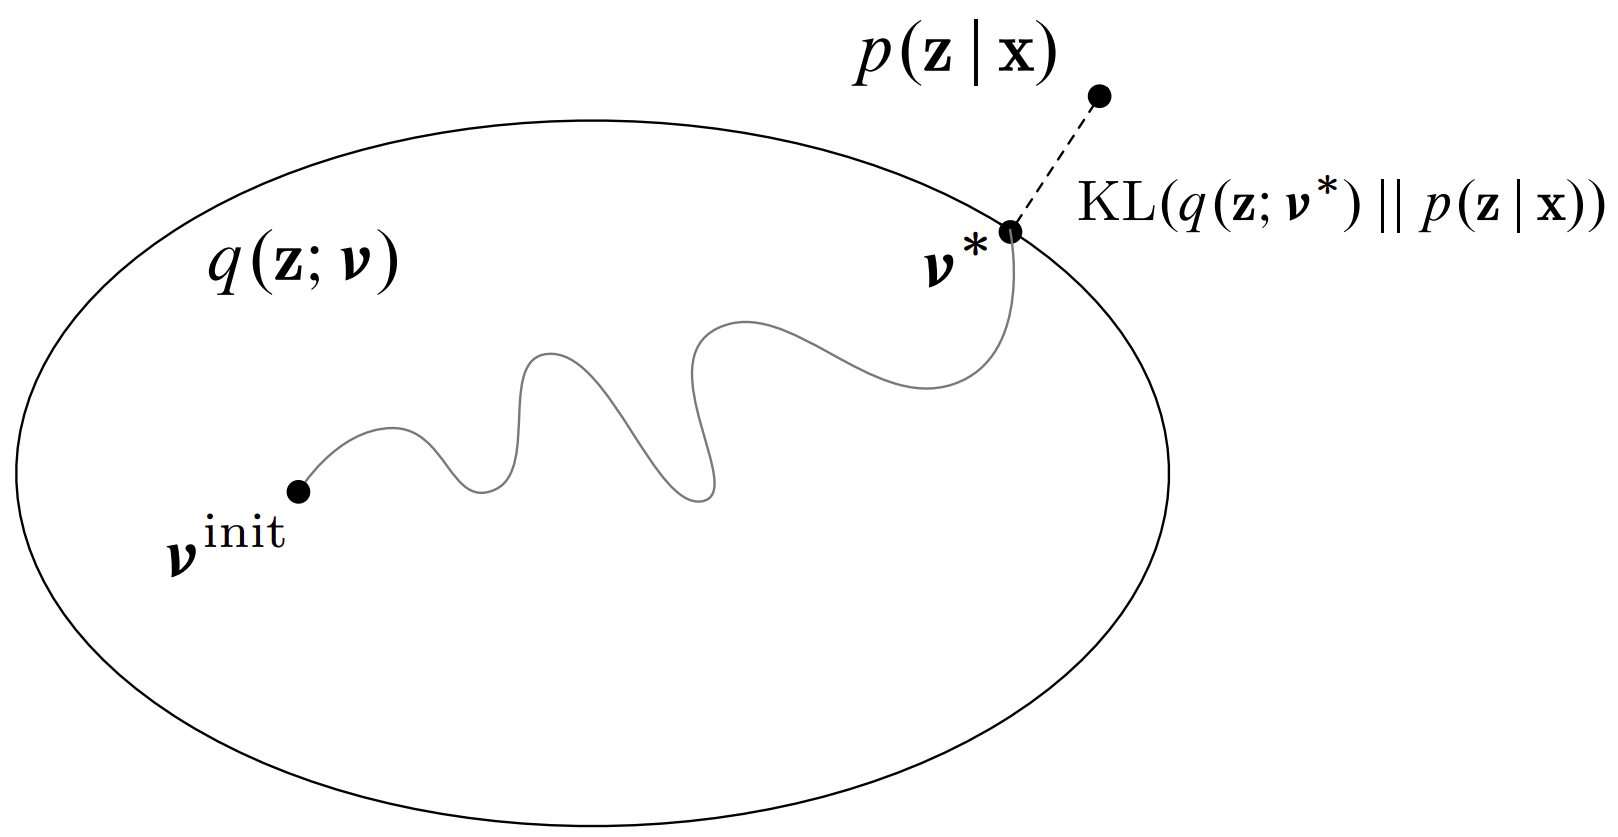
\includegraphics[width=0.5\textwidth]{figures/vi_illustration.png}
	\caption[Caption for LOF]{Illustration of \acrlong{vi}\footnotemark.}
	\label{fig:vi}
\end{figure}
\footnotetext{\url{http://www.cs.columbia.edu/~blei/talks/Blei\_VI\_tutorial.pdf}}

\subsubsection*{LDA learning}
We use an implementation of the \gls{lda} which is based on \cite{blei2010online}, where \citeauthor{blei2010online} present a way of training the \gls{lda} using \gls{vi}.
They do this by using stochastic \gls{vi}, which also outperforms batch learning.
In learning the \gls{lda}, we first sample a batch of documents from the whole corpus, where we learn the structure of this sample and use it to update the topics within the model.
To do this, we need some form of verification of whether we are getting closer to the the true posterior distribution $p(z|\textbf{x})$.
In \gls{lda}, we use perplexity as a score to check whether we are moving towards $p(z|\textbf{x})$
\todo{write a little section about how we change the elbo, and use that to try and approximate the true postiore}

\subsection{Problem With Using Perplexity in Hyperparameter Search}
In \autoref{subsec:hyperparameters}, the way we found the optimal hyperparameters for the \gls{lda} model is described.
There, it is described that we evaluated the models based on both perplexity and human evaluation.
Human evaluation was necessary because of the way perplexity is calculated for models.

The model that had the lowest perplexity of $202.913$ had the hyperparameters: $(K=15, \alpha =0.01, \eta =0.1)$.
In comparison, the model that was chosen for the experiment had a perplexity of $212.511$ and had the hyperparameters: $(K=30, \alpha =0.1, \eta =0.1)$.
If we used purely perplexity for choosing the hyperparameters for the model, we would have ended up using a model with 15 topics.
Instead we used both perplexity and human evaluation of the models, based on which models had the most humanly understandable topics.
Here we evaluated the models with the lowest perplexities for these K-values: 5, 10, 15, 20, 25, 30, and 35.
We did not look beyond 35, because the perplexity became significantly higher.\todo[inline]{Måske passer noget af dette bedre i gridsearch afsnittet.}
When looking at the most representative words of the first 5 topics in the 15-topic model, as seen in \autoref{fig:15TopicWords}, it is clear that what these topics cover is too wide.

\begin{figure}[h]
	\centering
	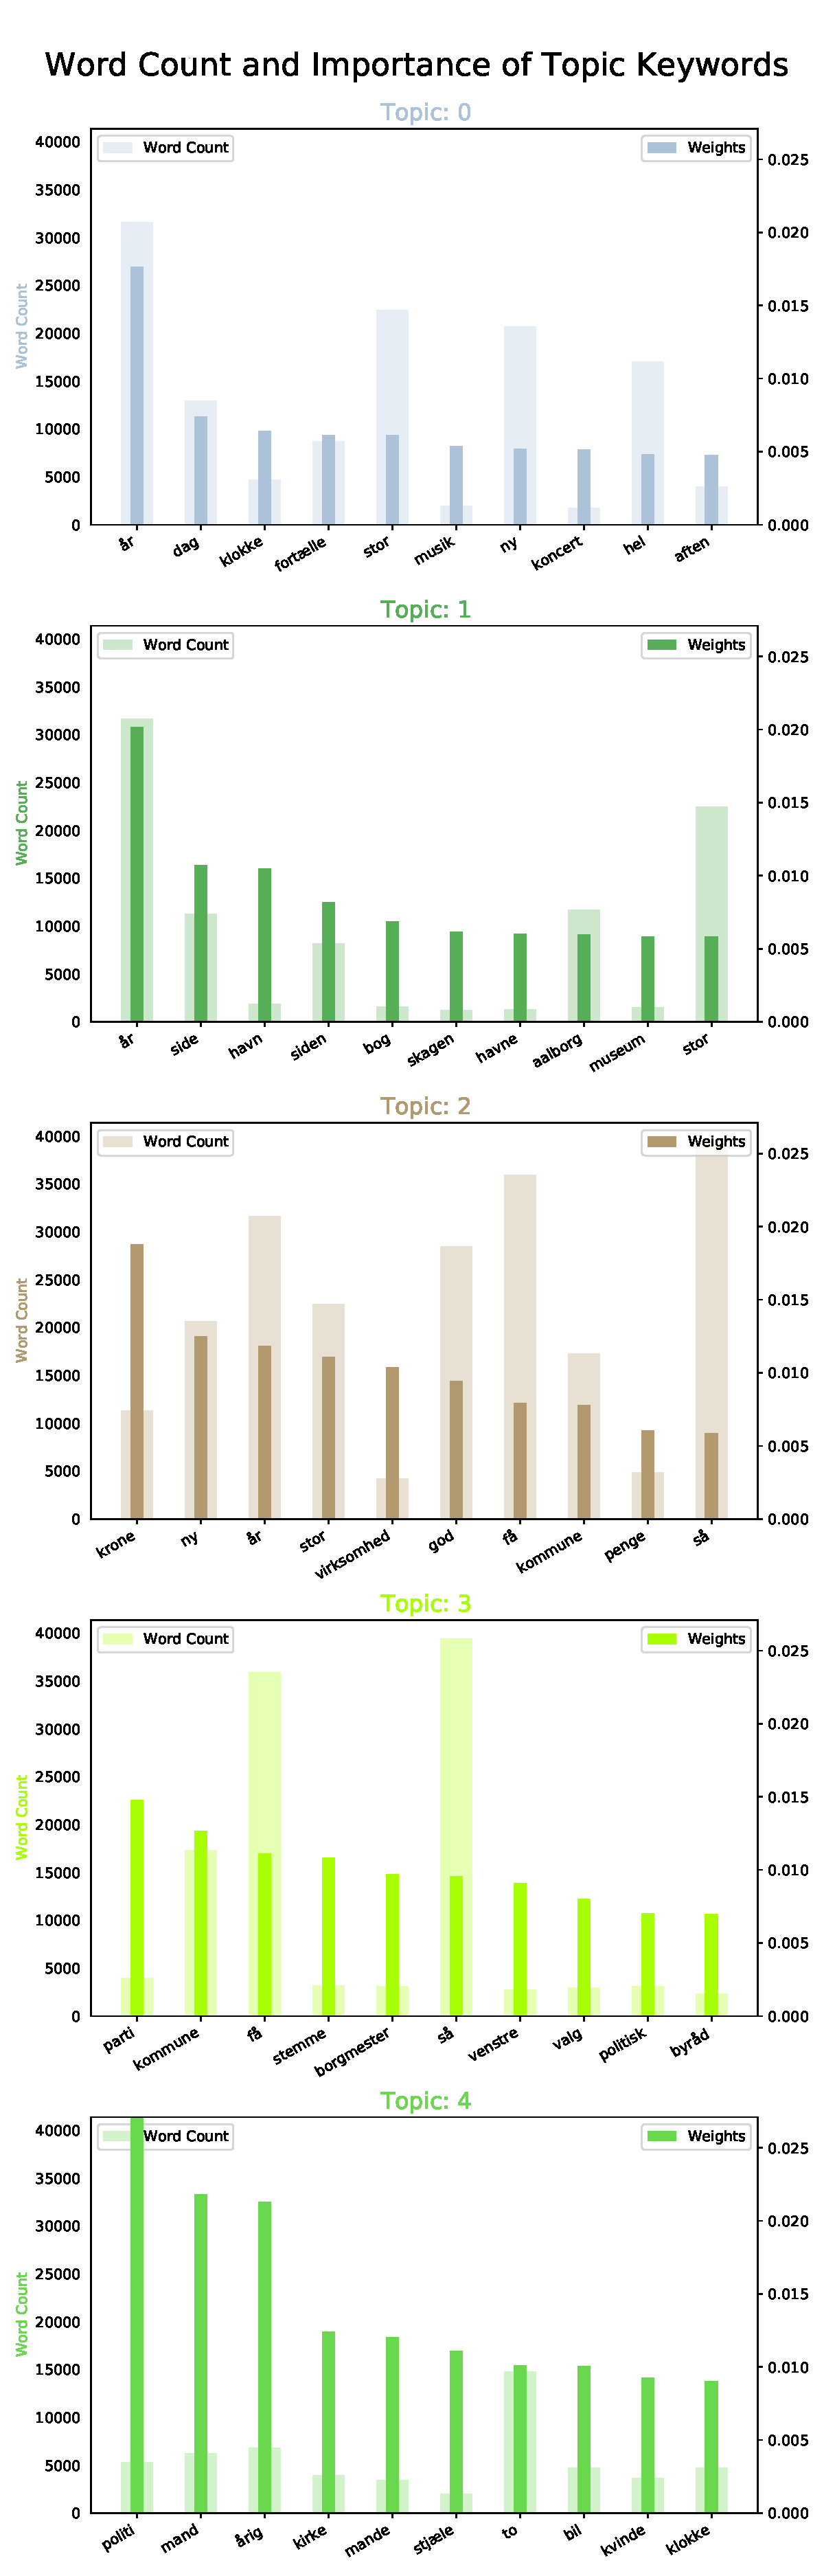
\includegraphics[width=0.45\textwidth]{figures/Word count and importance_corpus2017_document_model(15, 0.01, 0.1)(15, 0.01, 0.1)_topic 0-4.pdf}
	\caption{The first 5 topics from the 15-topic model.
	The most important words for each topic, sorted by the words weight in the topic, are shown.}
	\label{fig:15TopicWords}
\end{figure}

This indicates that the granulaty of the dataset at 15 topics is too low to give humanly understandable topics.
When looking at the most representative words of the first 5 topics in the 30-topic model, as seen in \autoref{fig:30TopicWords}, some more understandable topics can be seen.
Though, it can also be seen that while some topics in the 30-topic model are still difficult to interpret, other topics are much more understandable.

\begin{figure}[h]
	\centering
	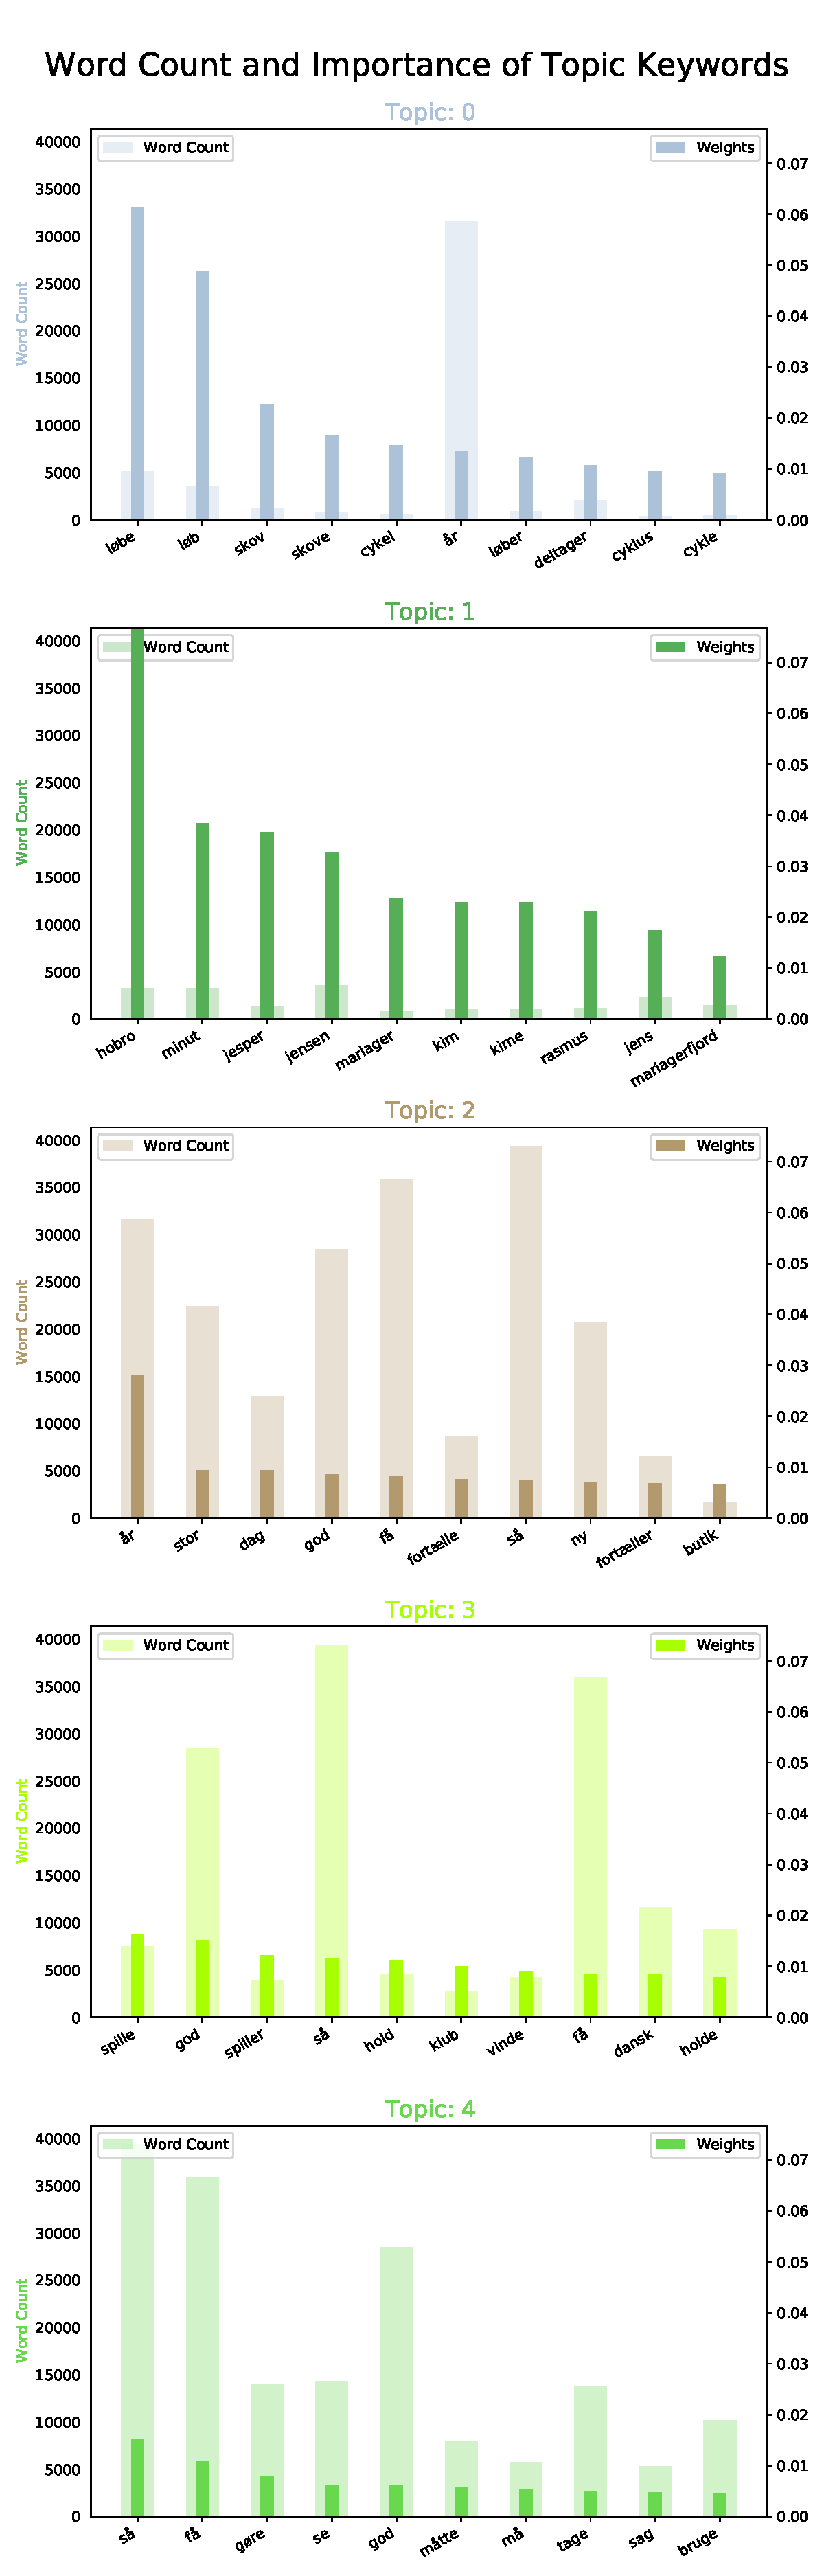
\includegraphics[width=0.45\textwidth]{figures/Word count and importance_corpus2017_final_model(30, 0.1, 0.1)(30, 0.1, 0.1)_topic 0-4.pdf}
	\caption{The first 5 topics from the chosen 30-topic model.
		The most important words for each topic, sorted by the words weight in the topic, are shown.}
	\label{fig:30TopicWords}
\end{figure}

This shows a conflict between using the best perplexity and having a good granularity, which is why perplexity by itself was evaluated to not be enough to choose the hyperparameters for the experiment.

\subsection{Representative documents for topics}

The weight is the probability of the document having been generated by a specific topic in the \gls{lda} model.
This is the topic with the highest probability from the topic probability distribution $\theta$ for the document.

\newpage
\onecolumn
	\begin{xltabular}{\linewidth}{@{}c|c|c|X@{}}
		\toprule
		{\footnotesize Topic} & {\footnotesize \thead{Document\\\#}} & {\footnotesize Weight} & {\footnotesize Document} \\
		\midrule
		0 & 30014 & 0.991 & "selv uden kalifatet vil is ise være en trusselselv uden kalifatet vil is ise være en trussel beirutte først røg ryge røge de ud af millionbyen mosul i irak og nu er jihadisterne fra islamisk stat is ise blive besejre i den syriske by raqqa raqqae der siden side har været hovedsæde for gruppe såkaldt kalifat men selv om is ise har miste stor del dele af sit fysiske territorie så vil der fortsat fortsætte være massere masse af udfordring i syrien og irak vurderer ekspert de advare samtidig om at is ise ideologi vil bestå og at gruppe støtter vil udgøre en terrortrussel i vesten vest den forfærdelig sandhed er at is ise vil være lige så livsfarlig en oprørsgruppe og farligt et terrornetværk som det var da det minded minde om en stat siger mellemøstekspert nicholas nichola heras fellow ved center for a new american security til nyhedsbureau reut udfordring er nu at is ise vil blive et hævngerrigt spøgelse der vil forsøge at skab skabe kaos fortsætter fortsætte han aymenn jawad al tamimi der forsker forske i jihadisme ved tænketank middle east forum er enig han forvente at islamisk stat vil fortsætte med at benytte sig af selvmordsbombere sprængladninger og have såkaldt sove celler rundtom i verden efter kalifatets sammenbrud angribe angreb i europa vil fortsætte noget tid endnu jeg tro at sejr over is ise som et statslignende projekt vil svække gruppe tiltrækningskraft men is ise vil have beirutte først røg ryge røge de ud af millionbyen mosul i irak og nu er jihadisterne fra islamisk stat is ise blive besejre i den syriske by raqqa raqqae der siden side har været hovedsæde for gruppe såkaldt kalifat men selv om is ise har miste stor del dele af sit fysiske territorie så vil der fortsat fortsætte være massere masse af udfordring i syrien og irak vurderer ekspert de advare samtidig om at is ise ideologi vil bestå og at gruppe støtter vil udgøre en terrortrussel i vesten vest den forfærdelig sandhed er at is ise vil være lige så livsfarlig en oprørsgruppe og farligt et terrornetværk som det var da det minded minde om en stat siger mellemøstekspert nicholas nichola heras fellow ved center for a new american security til nyhedsbureau reut udfordring er nu at is ise vil blive et hævngerrigt spøgelse der vil forsøge at skab skabe kaos fortsætter fortsætte han aymenn jawad al tamimi der forsker forske i jihadisme ved tænketank middle east forum er enig han forvente at islamisk stat vil fortsætte med at benytte sig af selvmordsbombere sprængladninger og have såkaldt sove celler rundtom i verden efter kalifatets sammenbrud angribe angreb i europa vil fortsætte noget tid endnu jeg tro at sejr over is ise som et statslignende projekt vil svække gruppe tiltrækningskraft men is ise vil have støtter i lange lang tid endnu siger tamimi ifølge nyhedsbureau afp islamisk stat sidde fortsat fortsætte på område i irak og syrien men primært i grænseområdet mellem de to land lande ifølge det amerikansk militær har is ise omkring kriger tilbage i område ved grænse er gruppe dog allerede under presse pres af del dels syriske regeringsstyrker med opbakning fra rusland del dels arabisk og kurdiske styrker der få får støtte støt af usa selv hvis det område som vente bliver befri vil is ise ekstreme tolkning af islam bestå mener charlie winter han er seniorforsker ved international centrum center centre for the study of radicalisation and political violence jeg tro ikke på at hvis man bare bar fjerne islamisk stats territorie så forsvinde islamisk stats ideologi siger han til afp charlie winter mener at is ise fortsat fortsætte se sig selv som en succes fordi gruppe har formå at udråbe et kalifat og holde det køre i flere år her blev der eksempelvis både båd lave lav lavet mønte mønt og udstede passe pas ingen anden har gøre noget ligne lignende i ny tid det vil mener han have en effekt på global jihadisme i årevis islamisk stat udråbe sit kalifat i juni siden side dengang har gruppe miste knappe knap procent af sit territorie ifølge en talsmand for den amerikanskledede koalition der bekæmpe gruppe i syrien og irak" \\
		\midrule
		1 & 29851 & 0.983 & "et skridte skridt nærmerecenter fem millioner kommunale krone hjælpe hjælper nationalparkcenter på veje vej thy forlig forlige om thisted kommune budget for har hjælpe nationalpark thy et pænt pæn skridte skridt nær nærmere virkeliggørelsen af plan om at opføre et nationalparkcenter i vorupør i kommune budget for er der afsætte et beløbe beløb på fem millioner krone til nationalpark stor formidlingsprojekt trædesten til natur hvor et nytte ny nationalparkcenter bliver en af nationalpark ansøgning fremgå at de fem millioner krone skulle bruge til nationalparkcentret vi er godt godte god tilfreds med at penge er afsætte til trædestens projektet som dække hele hel område siger torben juul olsen formand for nationalpark bestyrelse budget i millionklassen trædesten til natur har et budget på millioner nationalparkcentret med et budget på millioner krone er en del dele af projektet med vished for yderligere yderlig fem millioner kommunale krone oveni de fem som allerede er tildele i forme form af værdi af en grunde grund og parkeringsarealer i vorupør konstatere torben juul olsen at nationalpark nu er meget tæt tætte på at være i mål måle med bestræbelse for at finansiere det komme nationalparkcenter inklusive de fem millioner kommunale budget krone har nationalpark nu millioner krone ud af byggesummen på mio krone ud over thisted kommune har nationalpark selv nordea fond og støtteforening nationalpark thy bidrage bidrag til beløbe beløb endnu mangel mangle nationalpark thy en udmelding fra en foreløbig ikke navngive fond som er ansøge om at støtte støt byggeri af nationalparkcentret med mio krone vi regne med at få fond tilkendegivelse senest i begyndelse af siger torben juul olsen mangel mangle halv million falde den positiv ud mangel mangle krone beløbe beløb vente rejse af støtteforening nationalpark thy som har bidrage bidrag med en million og foreløbig har indsamle krone af den halv million nationalpark har søgt søge kommune om forlængelse af dispensationen fra naturbeskyttelseslovens paragraf til byggeri af centre centrum center i vorupør dispensationen er oprindelig givet give for tre år" \\
		\midrule
		2 & 5507 & 0.993 & "det ske tirsdag november øst øse vildsunde vildsund færgekro fremtid er digital infomøde om landbonords digitale løsning bankohall bankohal nykøbing lotterispil nykøbing kirke festkoncert med musica ficta og bo holten nykøbing kirkecenter højskoleaften ved pastor leiff hvass fjordglimte fjordglimt kom og synge bio men mens vi levere leve lever med krop og sjæle sjæl thor ragnarok foredrage foredrag sære sans sanse jigsaw onsdag november morsø kirkehøjskole ole dybro om reformationsmaleren luca cranach aktivitetshus i sejerslev banko ansgarshjem kortspil hvidbjerg plejecenter banko sundhedscenter i nykøbing cafe for kræftramt og samvær med anden arr morsø lokalforening kb støberigård virkelyst underholdning ved dorthe græsborg det ottekantet forsamlingshus øster jølby valgtræffe valgtræf arr morsø folkeblad og radio limfjord superbrugs øster jølby km motionstur arrangere af morsø fodslaw bio men mens vi levere leve lever med krop og sjæle sjæl thor ragnarok jigsaw indlæg indlægge til liste list skal sendes pr maile mail til redaktion mf dk og der skal stå det ske i emnefelt deadline er mandag klokke kl uge før føre din dit arrangement torsdag november johan rii minde strikkecafe johan rii minde gå tur ture støberigård banko med mulighed for hjælp hjælpe støberigård knipling m m rotary park torsdagsklub ansgarshjem knipling dansk skaldyrcenter tang hav planter plante foredrage foredrag morsø teater den glade enke gæstespille gæstespil operettekompagniet arr morsø teaterkreds bio victoria abdulle fantasten a bad bede bade moms momse christma jigsaw indlæg indlægge til liste list skal sendes pr maile mail til redaktion mf dk og der skal stå det ske i emnefelt deadline er mandag klokke kl uge før føre din dit arrangement fredag november støberigård åben aktivitetscenter ansgarshjem synge sang støberigård gymnastik på stole stol johan rii minde banko bio fantasten victoria abdulle the treasure hunt a bad bede bade moms momse christma jigsaw indlæg indlægge til liste list skal sendes pr maile mail til redaktion mf dk og der skal stå det ske i emnefelt deadline er mandag klokke kl uge før føre din dit arrangement lørdag november skarregaard julemarked bio den utrolig historie om den kæmpestor pære my little pony film sikken et cirkus victoria og abdulle fantasten a bad bede bade moms momse christma jigsaw indlæg indlægge til liste list skal sendes pr maile mail til redaktion mf dk og der skal stå det ske i emnefelt deadline er mandag klokke kl uge før føre din dit arrangement søndag november skarregaard julemarked sundbyvej thy morse mor husflid afholde husflidsmesse bankohall bankohal nykøbing lotterispil bio operabio norma den utrolig historie om den kæmpestor pære my little pony film sikken et cirkus victoria og abdulle fantasten a bad bede bade moms momse christma jigsaw indlæg indlægge til liste list skal sendes pr maile mail til redaktion mf dk og der skal stå det ske i emnefelt deadline er mandag klokke kl uge før føre din dit arrangement mandag november støberigård åben aktivitetscenter johan rii minde gymnastik ansgarshjem motion på stole stol støberigård vi hækle m m rotary park kortklub støberisal seniorbridge sprogskole i frøslev nordmor byorkester spiller spille midtmorse midtmor sport på vag vagt i afghanistan foredrage foredrag med peter fyllgraff vil fritidscenter banko bio victoria og abdulle fantasten glasslot a bad bede bade moms momse christma indlæg indlægge til liste list skal sendes pr maile mail til redaktion mf dk og der skal stå det ske i emnefelt deadline er mandag klokke kl uge før føre din dit arrangement tirsdag november ansgarshjem vi nørkle støberigård åben aktivitetscenter støberigård oplæsning og snakke snak udfra bog om egon plejdrup støberigård højskoleforedrag ved hans ole vester støberigård patchwork m m aktivitetshus i sejerslev besøge besøg af præst anna holck ansgarshjem gudstjeneste dansk skaldyrcenter østerssafari johan rii minde gudstjeneste smørdalsvej ljørslev forberedelse til juleværksted mørkehistorier m m arrangere af morsø naturklub bankohall bankohal nykøbing lotterispil støberisal julearrangement bio fantasten victoria og abdulle foredrage foredrag inspiration fra natur a bad bede bade moms momse christma indlæg indlægge til liste list skal sendes pr maile mail til redaktion mf dk og der skal stå det ske i emnefelt deadline er mandag klokke kl uge før føre din dit arrangement" \\
		\midrule
		3 & 24775 & 0.952 & "årig model rådgive rådgiver trump washington det hvid hvide hus hu huse har udnævne den årig hope hicks til den indflydelsesrige poste post som kommunikationschef det bekræfte sarah huckabee sanders der er talsperson for det hvid hvide hus hu huse hicks har i de sen uge arbejde som midlertidig kommunikationschef for den amerikansk præsident donald trump men nu er stilling blive faste fast den tidlig tidligere model og pr konsulent er tæt tætte på trump familie og har været rådgive rådgiver for donald trumps datter ivanka hun er den tredje kommunikationschef i det hvid hvide hus hu huse i løb løbe af otte måned ritzau ap" \\
		\midrule
		4 & 12748 & 0.995 & "rh ne er et sikkert sikker vælge til julemadenden kraftige vin lade lader sig ikke slå ud af rødkål og julesul vi har testet flotte vin vine og er imponere de røde rh ne vin vine er et godt godte god julevalg vi ved det for vi har selv dem smage og det kan betale sig at læg lægge en hundredekroneseddel eller to eller flere oven i det vin koster koste til daglig for generel stige oplevelse med prise pris det kunne nordjyske smagehold konkludere efter flaske rh ne fra nord til syde syd der var safte saft og kraft og massere masse af kvalitet rh ne er selvfølgelig et vidt vid begribe begreb der er kæmpe forskel på om man drikke den rene syrah fra hermitage i nord eller en c tes du rh ne lang længe sydpå eller en ch teauneuf du pape hvor der måtte må indgå forskellig drue men de du dur dure alle sammen til vores vi traditionel julemad med deres gode god rene garvesyrer og en solid struktur c tes du rh ne village c tes du rh ne famille perrin coudoulet de beaucastel smv krone point lidt lide parfumeret duft dufte frisk friske bærduft fylde godt godte god i mund temmelig krydre lidt lide tørt bid bide til sidst fin balance dom r m jeanne les legantiers village bichel krone point temmelig lukke men åbner åbne sig pænt pæn når den få får lufte luft i glas kan evt dekanteres en smule rustik i duften fin frugt frugte i smag god balance røde bær bære le bouquet des garrigues vinspecialisten krone point ren og klare klar duft dufte finte fint fin bid bide frisk friske og umiddelbar vin cairanne dom oratoire st martin les douyes bichel krone point flotte flot tæt tætte farve koncentrere duft dufte med hint hin af chokolade tæt tætte vin med god eftersmag krydre lidt lide lakrids og et godt godte god bid bide af fin garvesyrer cornas cornas alain verset bichel krone point lædere læder og urter i duften intens og tør tø turde tørre vin med godt godte god integrerede garvesyrer gigondas syterres de bois neuf vin vin krone point alder ses se i farve der har få et brunt skære skær det fornemmes også i duften med noter af modne moden blommer afrundet vin der ikke holde holder til for meget eddike i rødkålene le primitif vin vin krone point duft dufte af røde bær bære kraftig robust vin med flotte flot struktur la r f rence vin vin krone point frisk friske bouquet af bær bære delikat bløde blød garvesyrer delas les reinages vinspecialisten krone point lidt lide lukke i duften så den måtte må gerne dekanteres fin balance ren frugt frugte tør tø turde tørre god mineralitet flotte flot vin dom cayron philpson krone point der er fornemmelse af alder i duften fin balance forholdsvis lette let le vin domain brusset les hauts de montmirail smv krone point kraftig vin dyb farve stort stor ekstrakt den kan virkelig bære julemaden chateauneuf du pape sabon le secret des sabon meny krone point fulde fuld fart farte på duften af brombær og modne moden blommer alder er tydelig i smag er der modne moden blommer lakrids og afrundede tørre tør tanniner godt godte god udvikle vin flotte flot vin domaine santa duc la crau ouest bichel krone point lædere læder i duften skal dekanteres for at åbne åben sig kraftig temmelig ung vin med mange muskler ch de beaucastel smv krone point duft dufte af sort kirsebær elegant bourquet flotte flot struktur perfekt balance delikat vin xavier vignon arcane v le pape supervin krone point intens bouquet brombær og mynte lækker læk lække vin i perfekt balance tør tø turde tørre med nogen mineralitet forbavsende ung olivier lafont meny krone point fyldig vin med flotte flot mørke mørk bær bære i duften den fylde hele hel mund nærmest fed fede men alligevel elegant her er mange muskler clos saint jean vinspecialisten krone point ren flotte flot bouquet lækker læk lække frugt frugte i smag der var også en fornemmelse af chokolade sabon prestige meny krone point lædere læder og mynte i duften tør tø turde tørre intens og krydre vin flotte garvesyrer elegant xavier vignon la r serve supervin krone point jeg var glad for stil fra den producent fin balanceret duft dufte i den ung unge vin alt var i balance elegant xavier vignon cuv e anonyme supervin krone point starte lidt lide lukke efter en snurretur i glas åbne den sig finte fint fin med modne moden bærnoter flotte flot veludviklet vin xavier vignon chateauneuf du pape supervin krone point ung vin med lidt lide urter og mynte i duften delikat vin med flotte flot afrundede garvesyrer fin balance sabon r serve meny krone point elegant vin dejlig duft dufte af mørke mørk bær bære god mineralitet ch de vaudieu philipson wine krone point lukke i duften ved opskænkning men den åbne flotte flot i glas give den en tur ture i en karaffel det åbner åbne også smag markere markeret garvesyrer der kan spille finte fint fin sammen med den fede fed made mad sabon les olivets meny krone point fin frugt frugte i næse elegant bouquet god fylde i smag ch fortia cuv e du baron bichel krone point kirsebær i duften lidt lide frugtsødme i smag en meget ung og frisk friske vin med godt godte god integrerede garvesyrer c te rotie delas seigneur de maugiron vinspecialisten krone point ung vin duft dufte af mørke mørk bær bære god frugt frugte og afrundede garvesyrer den er lige til at drikke drik og det er forbavsende med syrah vin i den alder balance mellem rødkålene den fede fed made mad og vin er garantere et hitte hit patrick jasmin smv krone point elegant afbalanceret duft dufte af brombær og kirsebær i mund er det en kraftig sag med massere masse af garvesyrer der skal luftes godt godte god for at blive afrundet meget ung vin der kan klare klar al den julemad den kombinere med hermitage delas domaine des tourettes vinspecialisten krone point flotte flot duft dufte med noter af kaffe lækker læk lække vin med brombær i smag fin balance mineralsk intens garvesyre der er perfekt integrere nicolas perrin smv krone point flotte flot vin delikat duft dufte der er en anelse animalsk fin balance i smag brombær kaffe og fornemmelse af træ crozes hermitage les croix bichel krone point her er der syrah for alle penge både båd i duft dufte og smage smag temmelig parfumeret næste rå i duften ung druepræget vin den kan man rolig roligt anvende sammen med al den tunge tung julemad der var stor spredning i karaktergivningen" \\
		\bottomrule
	\end{xltabular}
\newpage
\twocolumn

\subsection{Encountered Problems}
\todo{indicate whether the problems were solved.}

\subsubsection{Too many low values}
The document-topic distributions seem to have too low entropy and a lot of very low values.
This causes each topic to have an average of $\sim$7000 docs in their distribution, however with very low entropy, meaning that some of these distributions are very insignificant, but still add space and time complexity to our sparse representations.
To fix this we try tuning a minimum threshold for a topic to be counted in the document-topic distributions, which can be set as a hyper-parameter for \emph{gensim.ldamodel.get\_document\_topics()}.
After setting up a minimum percent of 2.5\% for an entry to be included in the document distribution, the number of documents per topic fell to ~4800, removing more than 5 entries per document for a total of $\sim$350.000 entries deleted. 
This has overall made the matrices a lot more sparse, but we will still have to evaluate whether changing K is better.

\subsubsection{Empty Topics}
There are also a significant number of topics, which had words, but no assigned documents. 
These should be detected and removed, though their existence points towards a lower $K$ might be needed.

\subsubsection{Too Common Topics}
On the opposite end, we also have some topics which are so universal that almost all documents are included in this topic. 
This might be a sign that the preprocessing is not working well enough, or it might once again point at the need for a better K.
Alternatively, too general topics could be manually pruned after the LDA model has been run.

\subsubsection{Adjacency Matrix Construction}
Our adjacency matrix is based on whether documents share some topics in their topic distributions. 
This leads us to the problem of $D*D*T$ insertion operations into a sparse matrix with what was originally ~50.000 documents. (unknown)
We did a lot of preprocessing, which reduced this number eventually all the way down to ~30.000 documents, but it was too insignificant to solve anything. (~140 days)
However our similarity function is symmetric, so we cut the time in half by only constructing half of the adjacency matrix. (~69 days)
We then changed our algorithm to only consider documents that shared topics to the original documents, decreasing our time to D\*T\_d\*D\_t, where both of the new variables are reduced compared to the originals. (~48 days)
We also made the calculation multithreaded in order to reduce computation time. (~2,4 days)
Lastly, we changed to construct our matrix using the \emph{lil\_matrix} format, which has faster insertions.


The function get\_document\_topics might be needing the whole corpus since whenever we give it the query it returns the same two topics. 
These two topics are probably the two most general topics within the model which might spell trouble since we don't know how to remove these from the model.

\subsubsection{Dirichlets produce Non-Zero values}
We use distributions produced by the Dirichlets to construct our adjacency matrix and to convert queries into topic distributions. 
However as part of how LDA is designed it never has 0 values in its distribution values, only extremely low numbers.
This is not optimal for constructing an adjacency matrix, as it would result in a fully connected graph.
Adjusting $\alpha$ and $\eta$ will make the low values lower, and the high values higher, but the problem never disappears from this.
We have therefore introduced thresholds. 
These thresholds reduce all values lower than the threshold to zero in the document-topic matrix and topic-word matrix.
The new problem introduced by introducing thresholds is that the exact values of the thresholds are now added as extra hyper-parameters for our solution.



% Examples of tables and figure
%\input{examples.tex}

%\section{Unused Sections}
%\input{unusedSections/KnowledgeGraph.tex}
\end{document}
